\section{Piecewise-quadratic Model}
\label{sec:setup.quad}

In this section, the first model with similar characteristics to the original model is constructed.
This chapter only includes the constructed models on the ``good'' path.
\Cref{chap:app.models} lists other models that are not included in this chapter.

This first model has 4 branches that are all quadratic.
Hence, it is called the piecewise-quadratic model.
In the original model, the branches $F_\B$ and $F_\D$ are shaped more like cubic functions, but to keep the number of parameters reasonable, this model assumes only quadratic branches.
The model also has the same symmetry as the original model, and it is included explicitly in the model definition.
The state space of all constructed models is $[0, 1)$ instead of $[0, 2\pi)$ as in the original model.

\subsection{Model Definition}
\label{sec:setup.quad.def}

The model is defined as the map $x_{n+1} = f(x_n) \mod 1$.
Where $f$ is given by the following set of equations.
\begin{align}
	f(x) & = \begin{cases}
		         g(x)                             & \text{if } x < \frac{1}{2} \\
		         g(x - \frac{1}{2}) + \frac{1}{2} & \text{else}
	         \end{cases} \label{equ:quad.f}           \\
	g(x) & = \begin{cases}
		         g_L(x) = a_L \cdot x^2 + b_L \cdot x + c_L & \text{if } x < \frac{1}{4} \\
		         g_R(x) = a_R \cdot x^2 + b_R \cdot x + c_R & \text{else}
	         \end{cases} \label{equ:quad.g}
\end{align}

\Cref{equ:quad.f} explicitly states the discontinuity at $0$ and $\frac{1}{2}$.
It also explicitly states the symmetry of the model.
Each half of the model is then governed by \Cref{equ:quad.g}.
Here all the 6 parameters $a_L, a_R, b_L, b_R, c_L,$ and $c_R$ act.
This equation also explicitly states the border at $\frac{1}{4}$.
And in combination with the explicit symmetry in \Cref{equ:quad.f}, the border at $\frac{3}{4}$ follows.

\subsection{Centered Parabola-shaped Branches}
\label{sec:setup.quad.even}

\hl{This section examines the piecewise-quadratic model with the centered parabola-shaped branches, see the functions in} \Cref{fig:setup.quad.even.cobwebs}.
\hl{
	To center the parabola-shaped branches, the parameter values $a_L = a_R = 6$, $b_L = -\frac{3}{2}$, and $b_R = -\frac{9}{2}$ are chosen and only the parameters $c_L$ and $c_R$ are varied.
	Both varied parameters are in the ranges $[0.25, 0.6]$.
}


This emulates the effect that $\chi_0$ has on the branches $F_\A$ and $F_\C$.
Increasing $c_L$ increases the values of the branches $f_\A$ and $f_\C$.
\hl{
	The effects of $E_0$ on branches $F_\B$ and $F_\D$ are lowering the values of the function on the left sides of the branches, moving the local minima of the branches to the left, and reducing the value of the function at the minima.
}
Decreasing $c_R$ does not have the same effects \hl{on the branches $f_\B$ and $f_\D$} but rather lowers the \hl{values of the function for} the whole branches.
\Cref{fig:setup.quad.even.period.full} \hl{shows 2D scans of the periods associated with parameter regions in this model}.

\begin{figure}
	\centering
	\subfloat[Full]{
		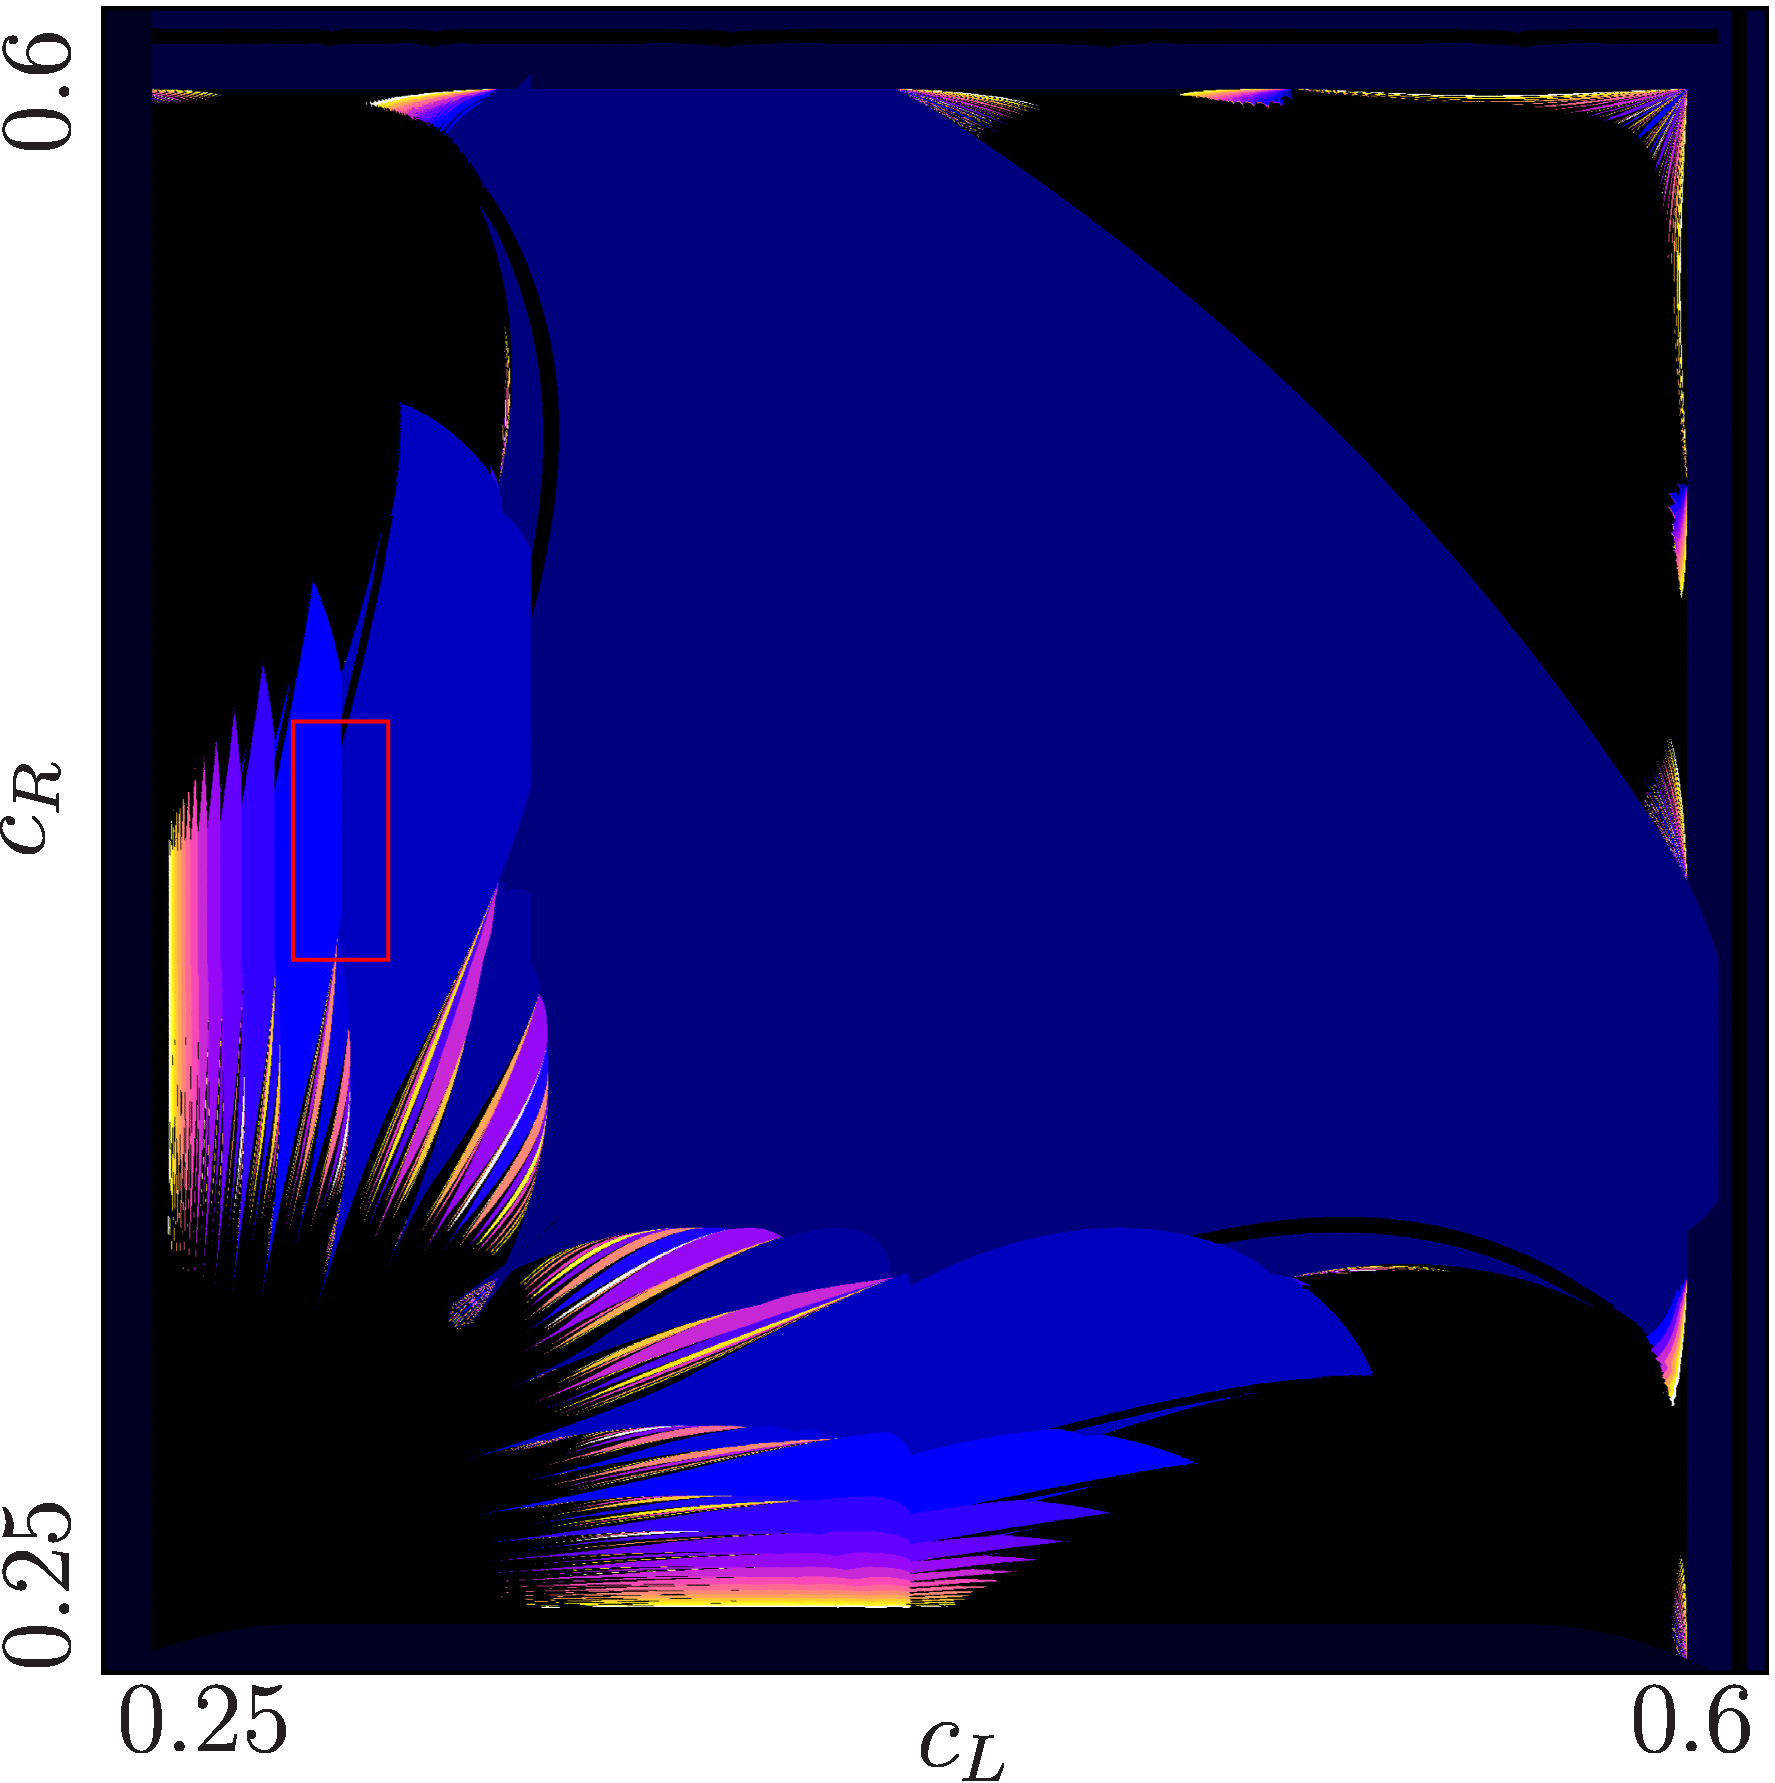
\includegraphics[width=.48 \textwidth]{../Figures/5/5.5a/result.png}
		\label{fig:setup.quad.even.period.full}
	}
	\subfloat[Zoomed]{
		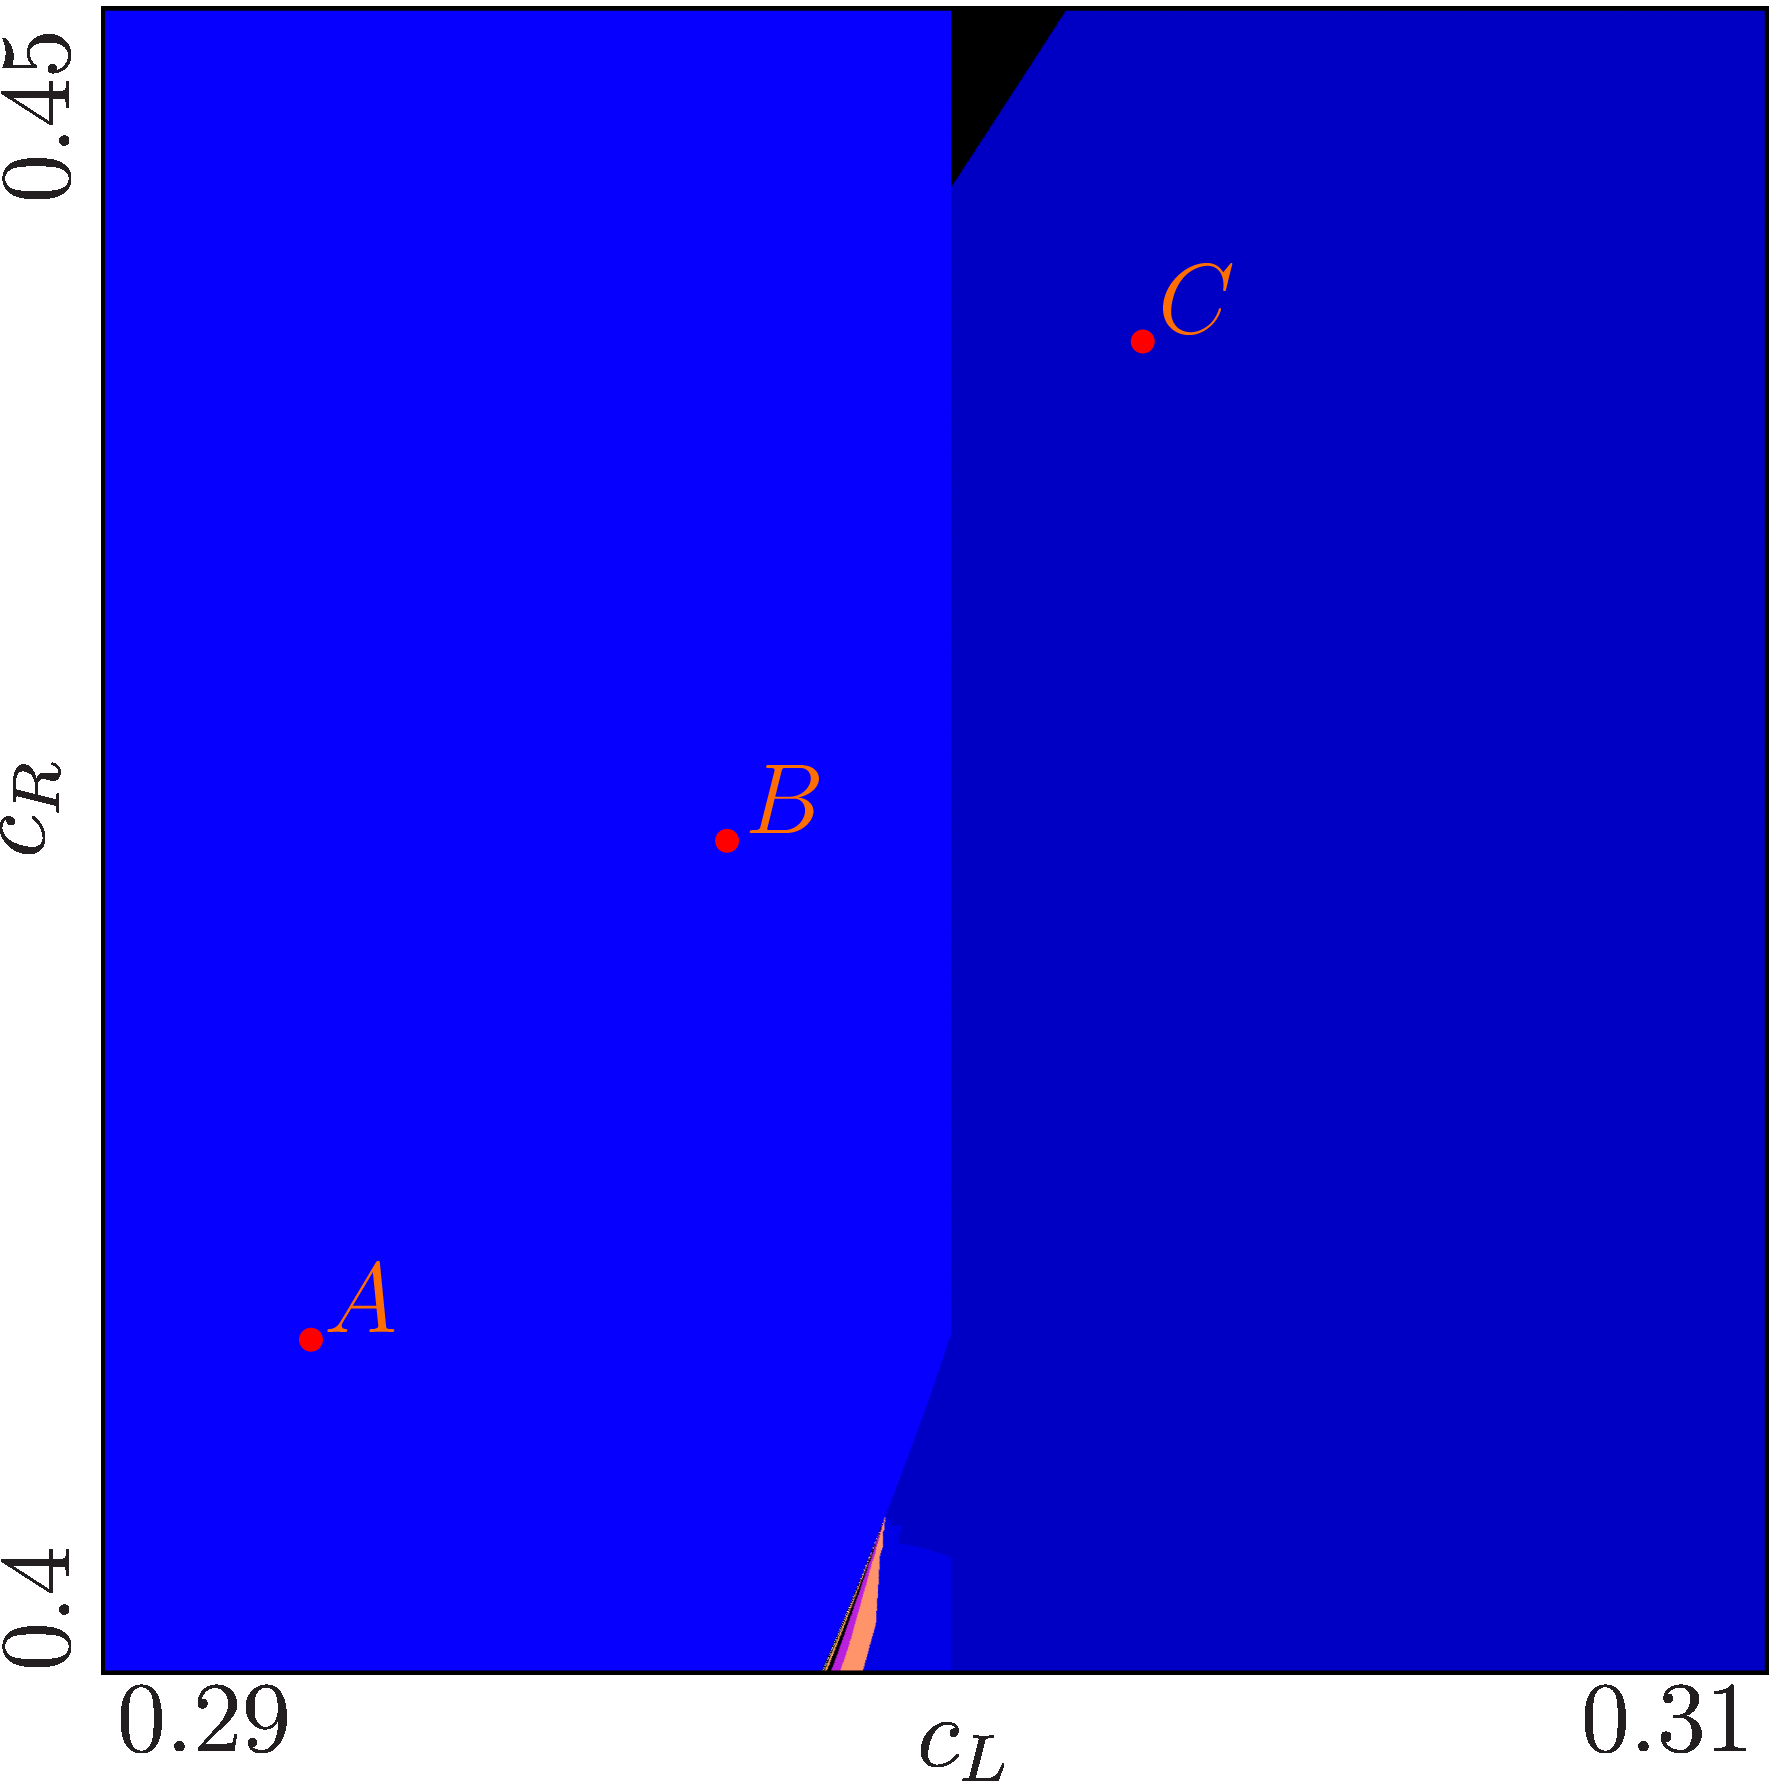
\includegraphics[width=.48 \textwidth]{../Figures/5/5.5b/result.png}
		\label{fig:setup.quad.even.period.zoomed}
	}
	\caption[2D scans showing periods of the even piecewise quadratic model]{
		2D scans showing the periods of the \hl{piecewise-quadratic} model with fixed parameters $a_L = a_R = 6$, $b_L = -\frac{3}{2}$, and $b_R = -\frac{9}{2}$.
		(a) shows the full structure with parameters $c_L$ and $c_R$ varied in the range $[0.25, 0.6]$ each.
		The red rectangle marks the parameter range that \hl{is shown magnified in} (b).
		The marked points in (b) are the parameter values for the \hl{cobweb diagrams} in \Cref{fig:setup.quad.even.cobwebs}
	}
\end{figure}

\begin{figure}
	\centering
	\subfloat[$A$]{
		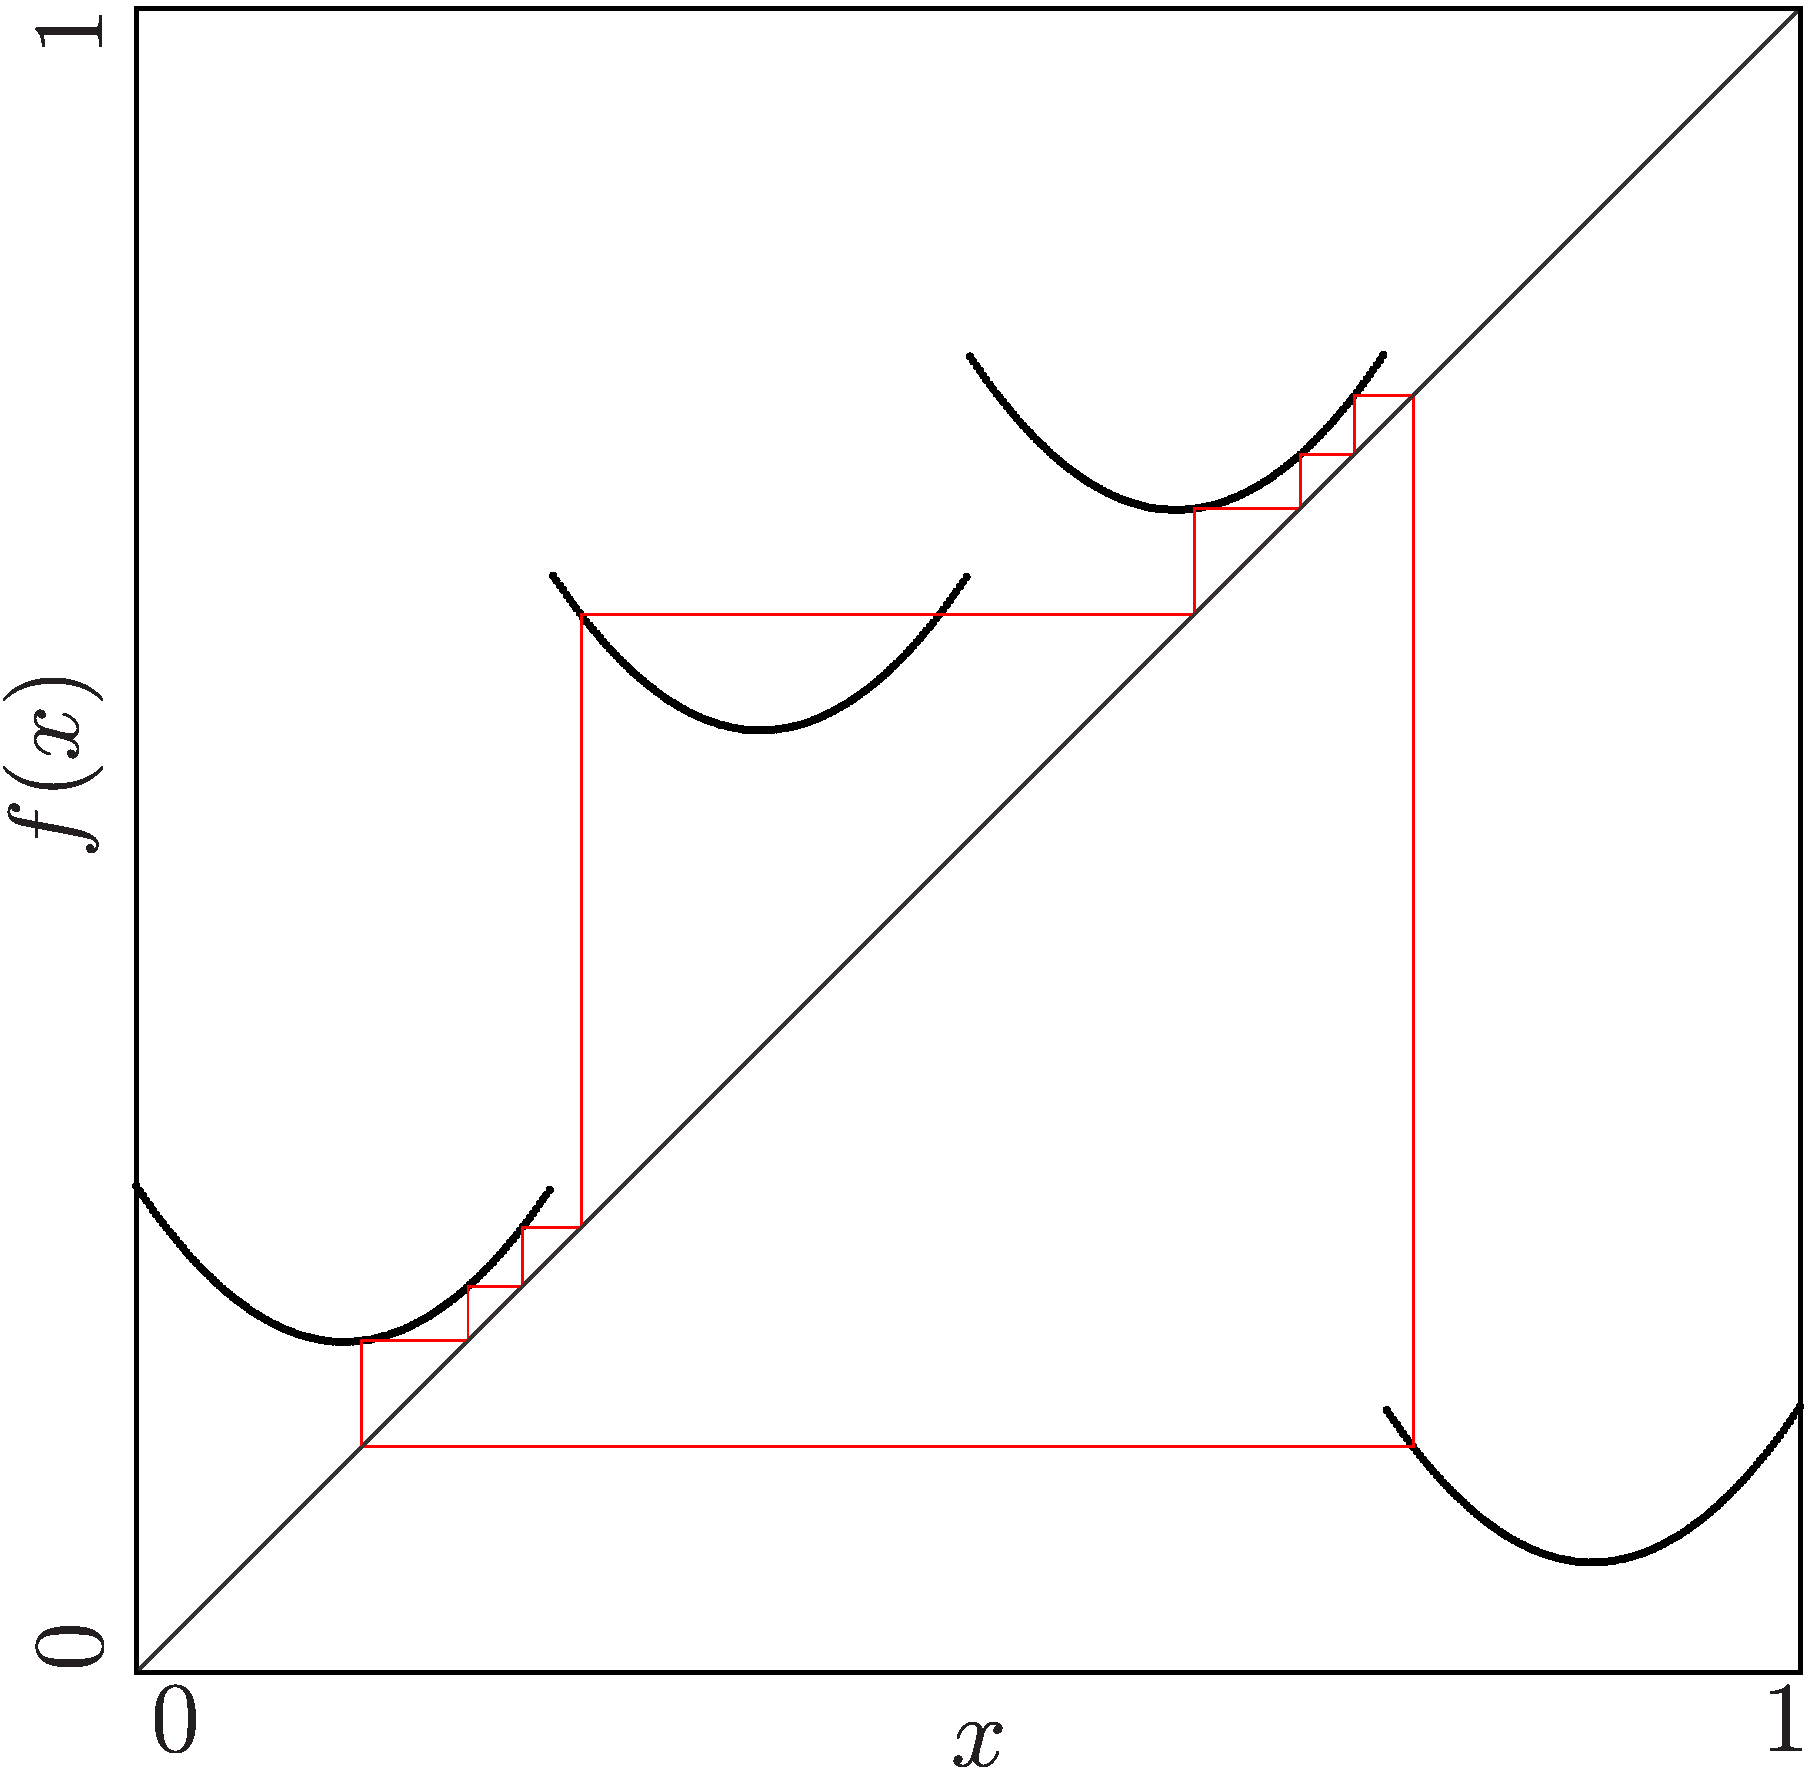
\includegraphics[width=.3 \textwidth]{../Figures/5/5.6a/result.png}
		\label{fig:setup.quad.even.cobweb.A}
	}
	\subfloat[$B$]{
		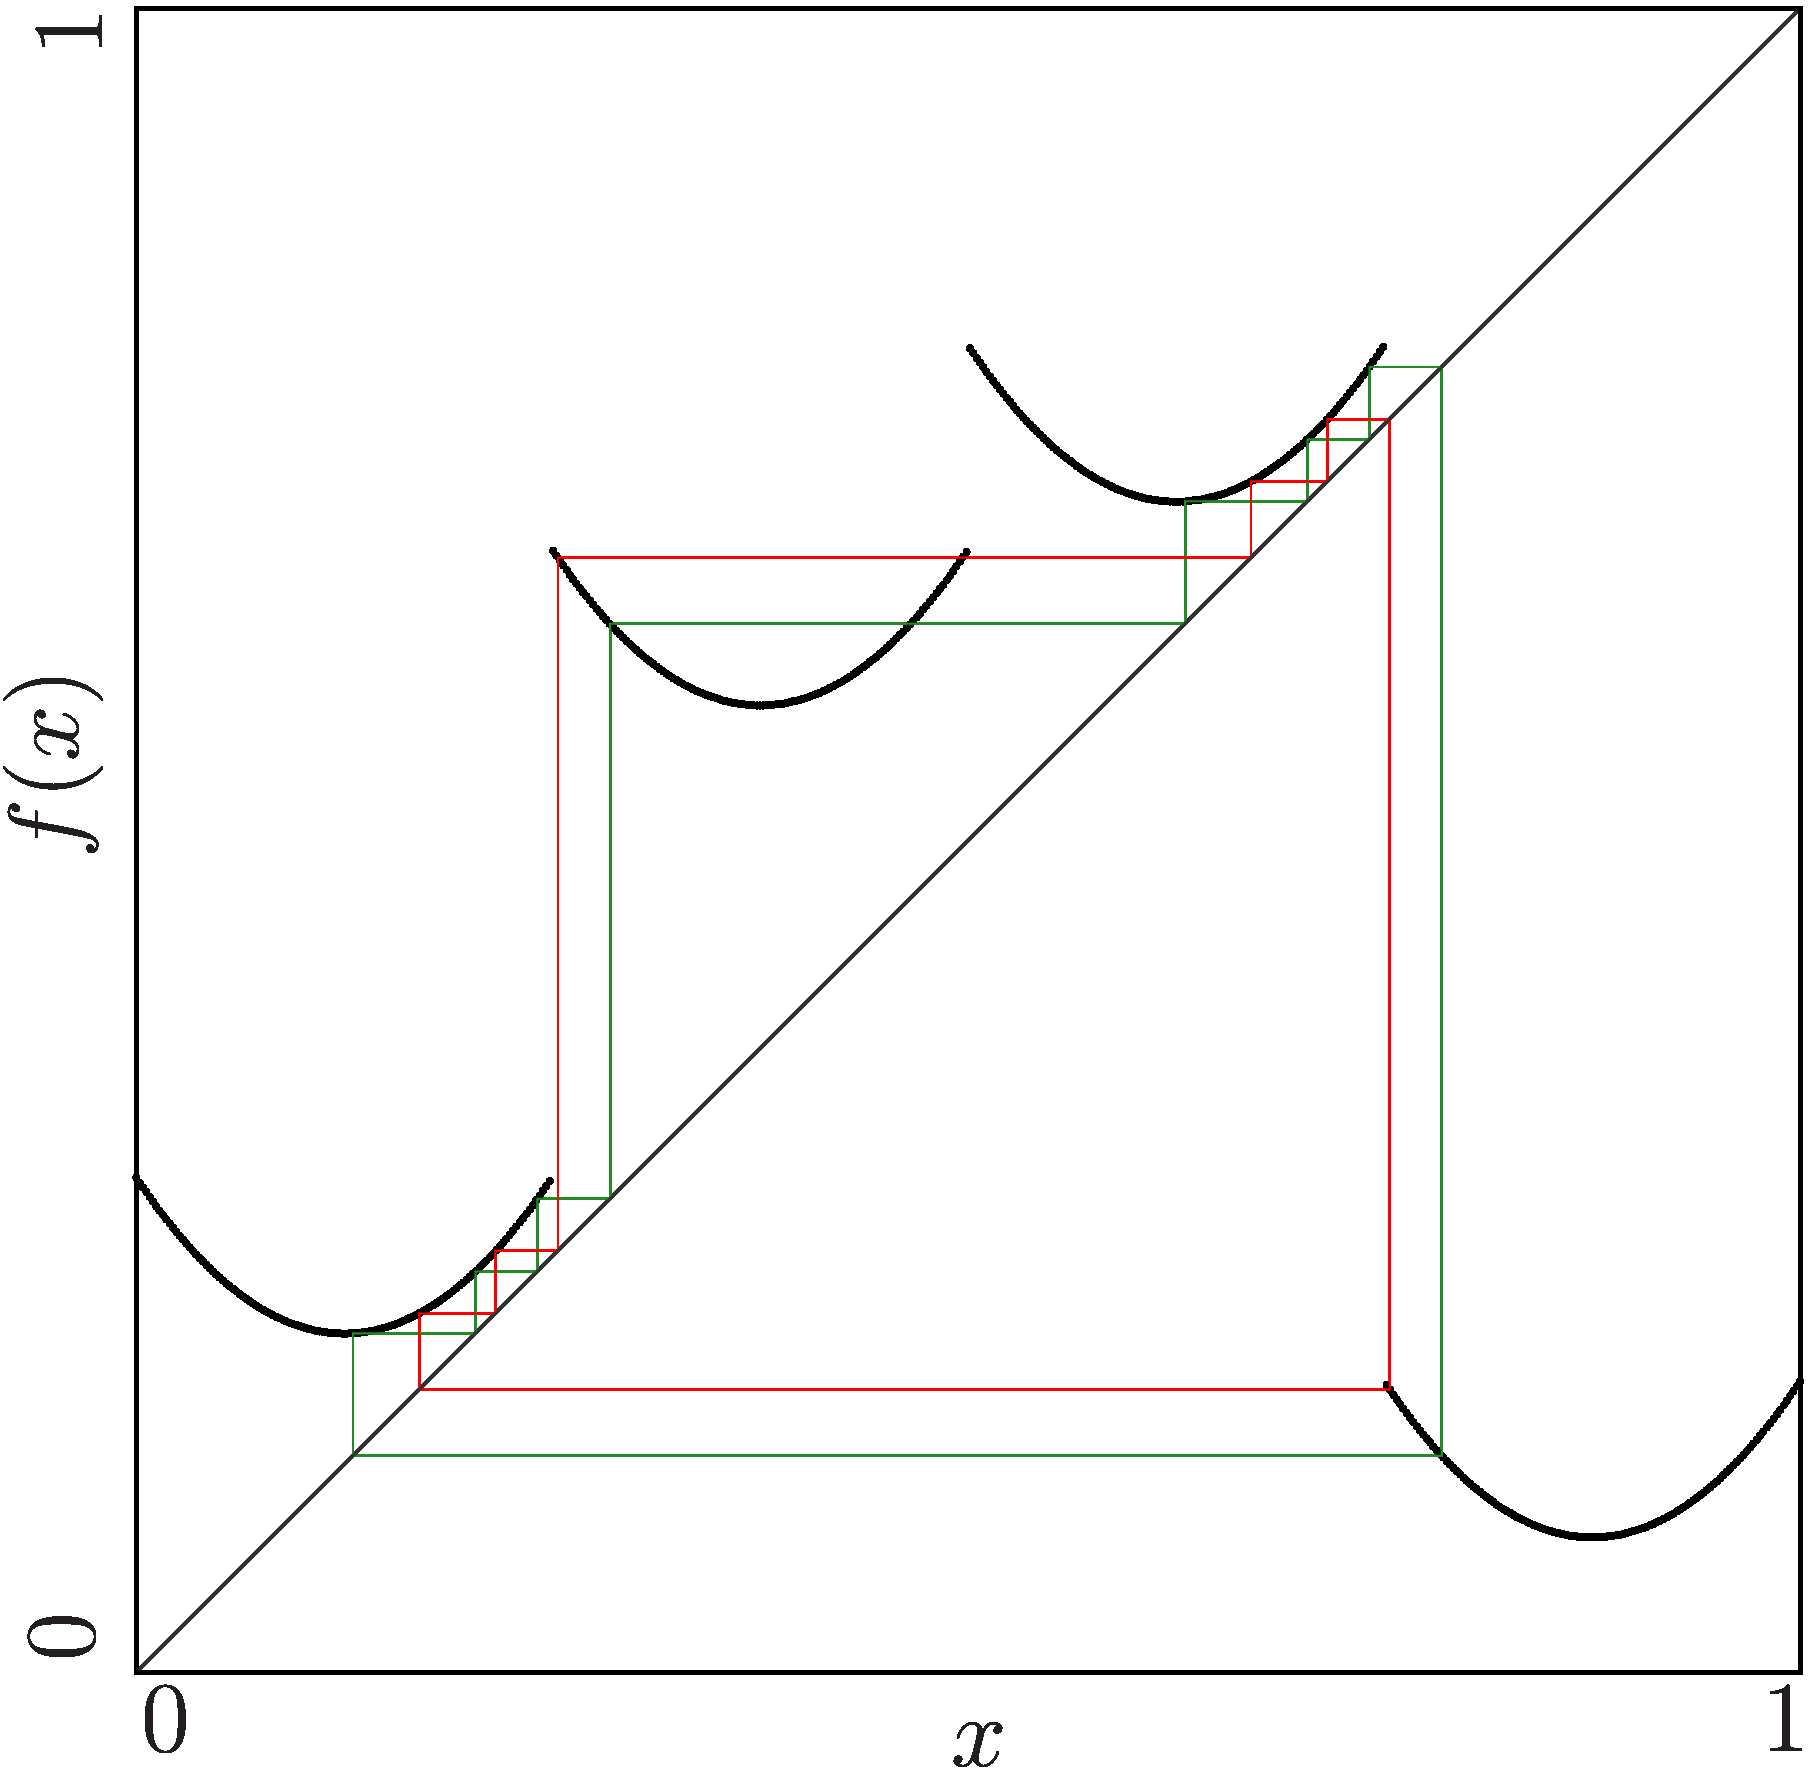
\includegraphics[width=.3 \textwidth]{../Figures/5/5.6b/result.png}
		\label{fig:setup.quad.even.cobweb.B}
	}
	\subfloat[$C$]{
		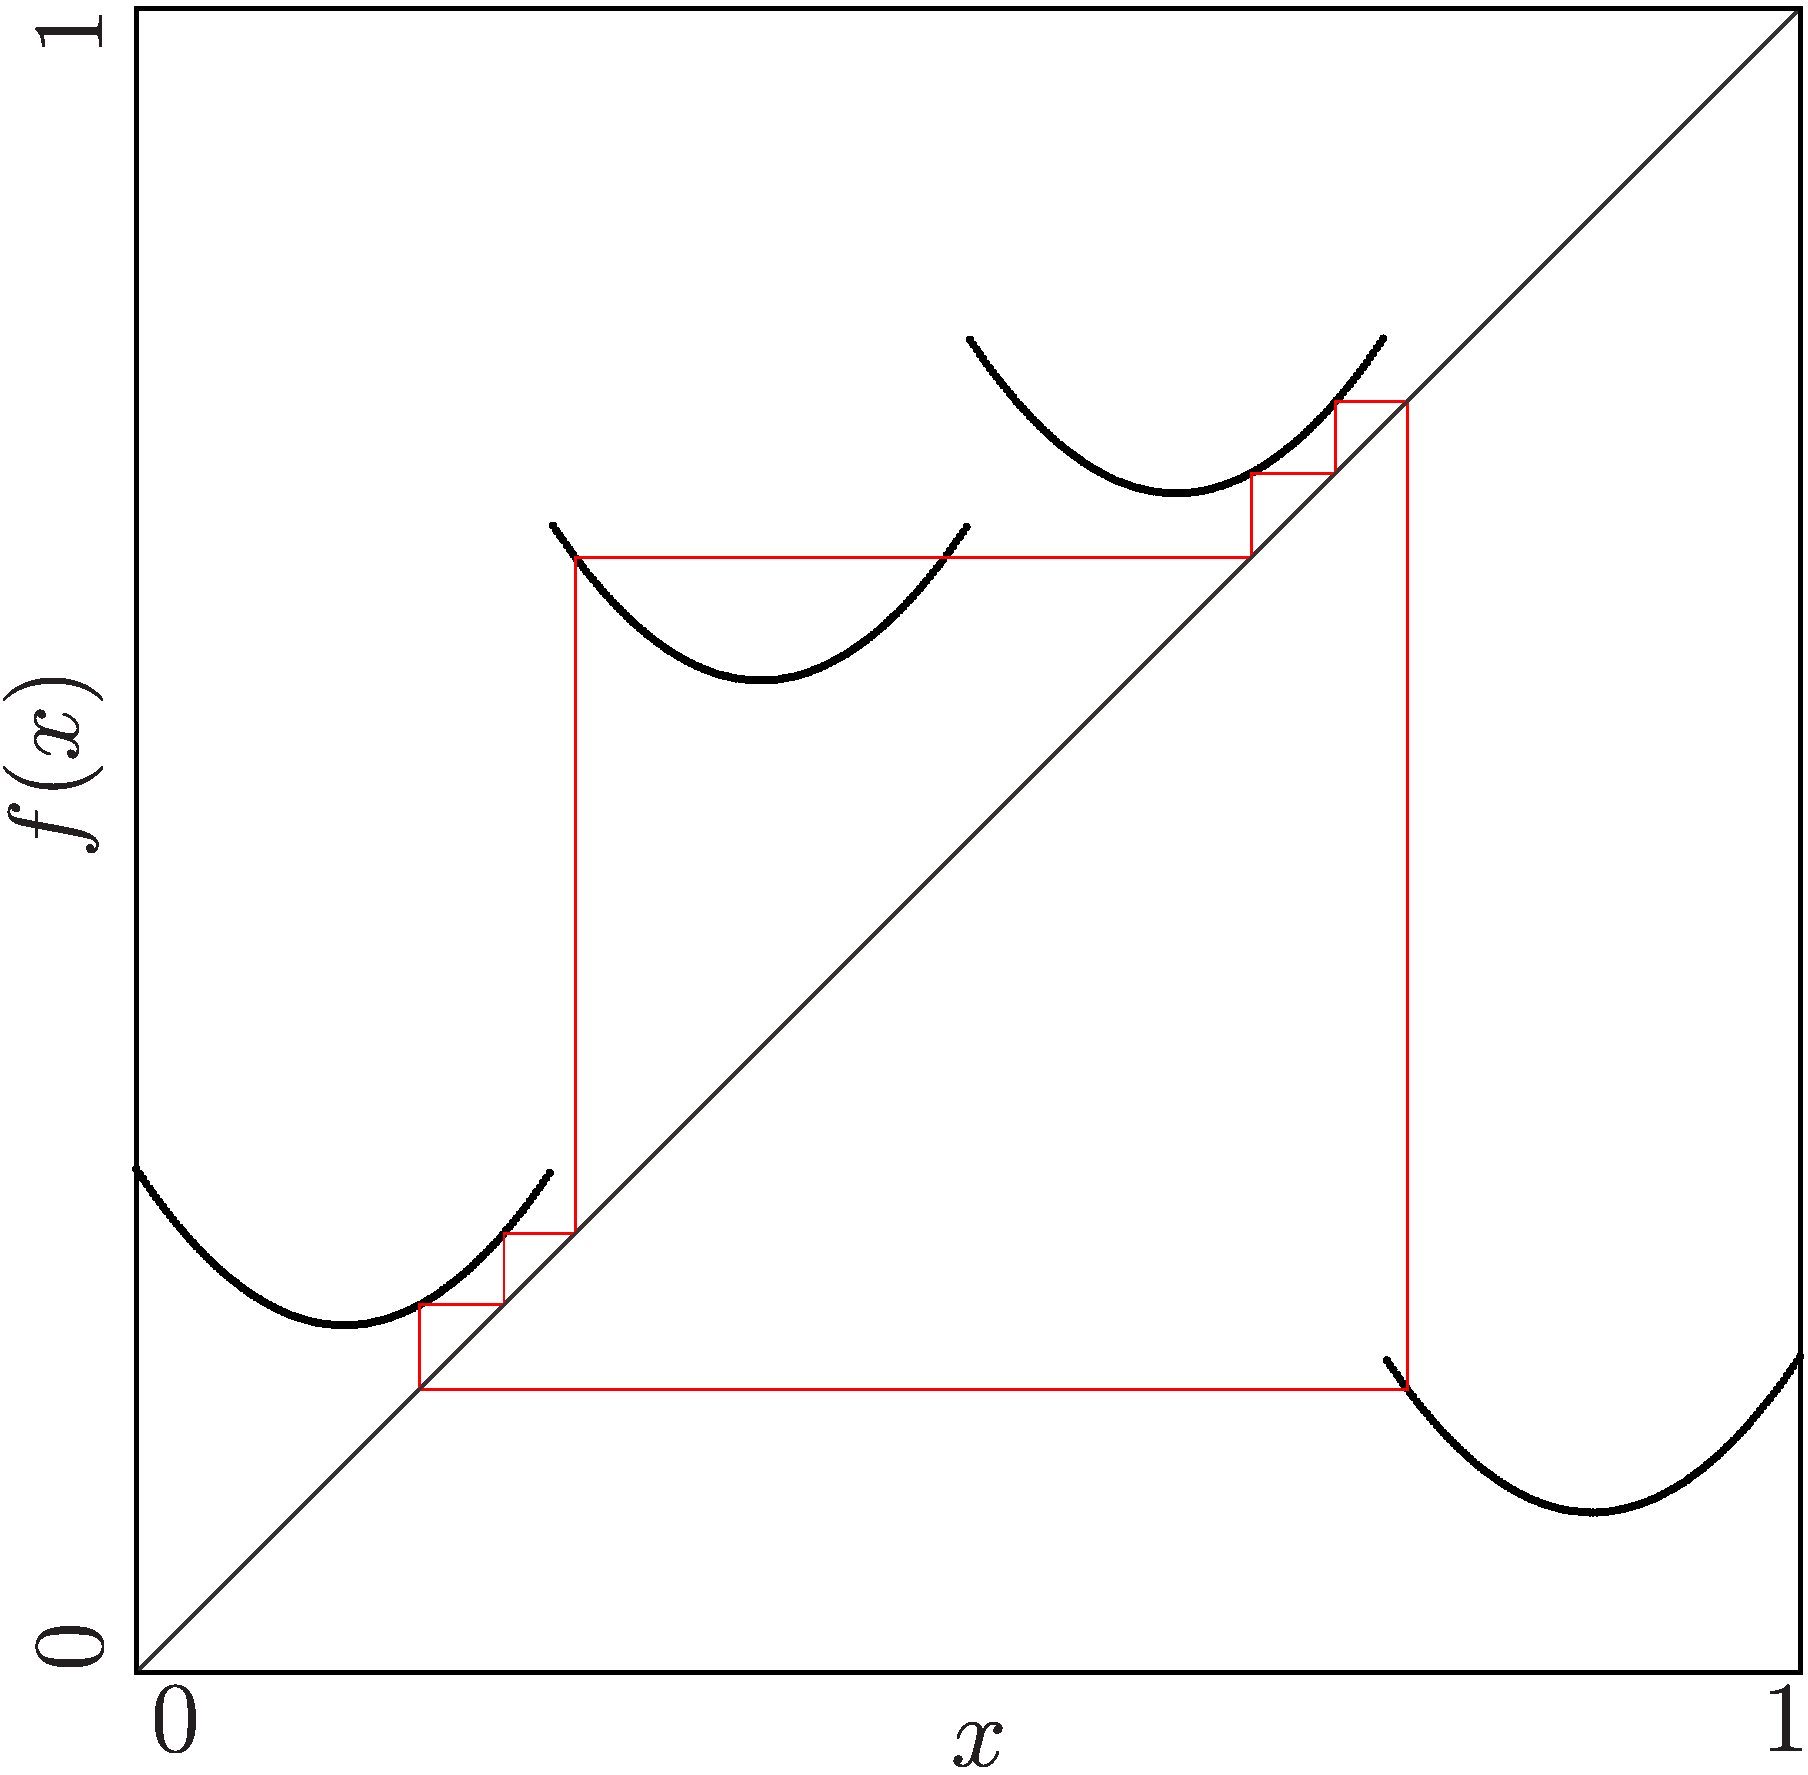
\includegraphics[width=.3 \textwidth]{../Figures/5/5.6c/result.png}
		\label{fig:setup.quad.even.cobweb.C}
	}
	\caption[Cobweb diagrams of the even quadratic model]{
		Cobweb diagrams at three parameter values of $c_L$ and $c_R$ in the piecewise quadratic model with fixed parameters $a_L = a_R = 6$, $b_L = -\frac{3}{2}$, and $b_R = -\frac{9}{2}$.
		The parameter values are marked \hl{with the points $A, B,$ and $C$} in \Cref{fig:setup.quad.even.period.zoomed}.
		(a) shows the cycle $\Cycle{\A^3\B\C^3\D}$ at \hl{the} point $A$ \hl{where $c_L = 0.2925$ and $c_R = 0.41$},
		(b) shows the two coexisting cycles $\Cycle{\A^3\B\C^3\D}$ (green) and $\Cycle{\A^2\B\C^2\D}$ (red) at the point $B$ \hl{where $c_L = 0.2975$ and $c_R = 0.425$},
		and (c) shows the cycle $\Cycle{\A^2\B\C^2\D}$ at the point $C$ where \hl{$c_L = 0.3025$ and $c_R = 0.44$}.
	}
	\label{fig:setup.quad.even.cobwebs}
\end{figure}

A phenomenon like in the original model \hl{can} not be found here.
But something very similar happens at the border of these wings.
\Cref{fig:setup.quad.even.cobwebs} shows the cobwebs at the points marked in \Cref{fig:setup.quad.even.period.zoomed}.
At point $A$, there is one stable cycle with period $8$.
This cycle is depicted in \Cref{fig:setup.quad.even.cobweb.A} and its symbolic sequence is $\A^3B\C^3\D$.
Point $B$ is in a parameter region, where 2 stable cycles coexist.
\hl{One can not} see this in the 2D scans in \Cref{fig:setup.quad.even.period.full}, since it only ever picks up on one cycle.
\Cref{fig:setup.quad.even.cobweb.B} shows the coexisting cycles at this border.
\hl{
	The symbolic sequences of the two coexisting cycles are $\A^3B\C^3\D$ and $\A^2\B\C^2\D$.
}
In contrast to the original model, the cycle that existed before in \Cref{fig:setup.quad.even.cobweb.A} \hl{with the symbolic sequence $\A^3B\C^3\D$} still exists alongside the new cycle with \hl{the symbolic sequence $\A^2\B\C^2\D$}.
\hl{
	At point $C$, there is again only one stable cycle.
	It has the period $6$ and the symbolic sequence $\A^2\B\C^2\D$.
	Therefore, this is the cycle that coexisted with the cycle with the symbolic sequence $\A^3B\C^3\D$ at point $C$.
}

This is different from the dynamics in the original model in two ways.
First, the cycles before and after the \hl{parameter region} of coexistence have different periods.
And second, the cycles existing outside the \hl{parameter region} of coexistence still exist inside the \hl{parameter region} of coexistence.
In the original model, the cycles existing outside the \hl{parameter region} of coexistence would disappear at the boundaries and new cycles would emerge inside this \hl{parameter region}.
Here, \hl{one} simply observes two overlapping parameter regions which is something different from the original model.

\subsubsection{Varying $c_L$ and $c_R$ while fixing $a_L = a_R = 6$, $b_L = -\frac{1}{2}$, and $b_R = -\frac{7}{2}$}

Choosing to make the parabolas centered was not ideal.
When looking at the original model function, one can see that the parabolas are not centered.
All branches are more skewed to the right.
To imitate this shape better, we now set $b_L = -\frac{1}{2}$ and $b_R = -\frac{7}{2}$.
All other fixed parameters are the same as above.
The parameters $c_L$ and $c_R$ are varied in the intervals $[0.08, 0.525]$ and $[0.825, 1.275]$, respectively, to capture a full structure.
\Cref{fig:setup.quad.even.period.full} shows a 2D scan of the periods of the stable cycles in this parameter range.
The structure seen in this figure repeats in all directions.

An interesting parameter area is marked with a red rectangle.
In this parameter area, 2 wings with the same period connect.
\Cref{fig:setup.quad.skew.period.zoomed} shows the 2D scan of the periods for this parameter range.
The points indicate the parameter values for the cobweb analysis.

\begin{figure}
	\centering
	\begin{subfigure}{0.4\textwidth}
		\centering
		\includegraphics[width=\textwidth]{21_Quadratic_mod1/Skew/S_2D_Period_Zoomed1/result.png}
		\caption{Full}
		\label{fig:setup.quad.skew.period.full}
	\end{subfigure}
	\begin{subfigure}{0.4\textwidth}
		\includegraphics[width=\textwidth]{21_Quadratic_mod1/Skew/S_2D_Period_Zoomed2/result.png}
		\caption{Zoomed}
		\label{fig:setup.quad.skew.period.zoomed}
	\end{subfigure}
	\caption[2D scans showing periods of the skewed piecewise quadratic model]{
		2D scans showing the periods of the piecewise quadratic model with fixed parameters $a_L = a_R = 6$, $b_L = -\frac{1}{2}$, and $b_R = -\frac{7}{2}$.
		(a) Shows the full structure with parameters $c_L$ and $c_R$ being varied in the ranges $[0.08, 0.525]$ and $[0.825, 1.275]$, respectively.
		The red rectangle marks the parameter range of (b).
		The marked points in (b) are the parameter values for the cobwebs in \Cref{fig:setup.quad.skew.cobwebs}
	}
	\label{fig:setup.quad.skew.period}
\end{figure}

\begin{figure}
	\centering
	\begin{subfigure}{0.3\textwidth}
		\centering
		\includegraphics[width=\textwidth]{21_Quadratic_mod1/Skew/S_Cobweb_A/result.png}
		\caption{At point $A$}
		\label{fig:setup.quad.skew.cobweb.A}
	\end{subfigure}
	\begin{subfigure}{0.3\textwidth}
		\centering
		\includegraphics[width=\textwidth]{21_Quadratic_mod1/Skew/S_Cobweb_B/result.png}
		\caption{At point $B$}
		\label{fig:setup.quad.skew.cobweb.B}
	\end{subfigure}
	\begin{subfigure}{0.3\textwidth}
		\centering
		\includegraphics[width=\textwidth]{21_Quadratic_mod1/Skew/S_Cobweb_C/result.png}
		\caption{At point $C$}
		\label{fig:setup.quad.skew.cobweb.C}
	\end{subfigure}
	\caption[Cobwebs of the skewed piecewise quadratic model]{
		Cobweb diagrams at three parameter values of $c_L$ and $c_R$ in the piecewise quadratic model with fixed parameters $a_L = a_R = 6$, $b_L = -\frac{1}{2}$, and $b_R = -\frac{7}{2}$.
		The parameter values are marked in \Cref{fig:setup.quad.even.period.zoomed}.
	}
	\label{fig:setup.quad.skew.cobwebs}
\end{figure}

\Cref{fig:setup.quad.skew.cobwebs} shows all the cobwebs taken at the points marked in \Cref{fig:setup.quad.skew.period.zoomed}.
The cobweb at point $A$ is shown in \Cref{fig:setup.quad.skew.cobweb.A}.
We can see that it has period 12 and its symbolic sequence is $\A^4\B^2\C^4\D^2$.
The cycle at point $C$ also has period 12.
Its cobweb diagram is shown in \Cref{fig:setup.quad.skew.cobweb.C}, and we can see that its symbolic sequence is $\A^3\B^3\C^3\D^3$.

From point $A$ to point $C$, one point of the cycle on the branch $f_\A$ moved to the branch $f_\B$.
The same thing happened to a point of the cycle on the branch $f_\C$, it moved to the branch $f_\D$.
This is similar to what happens in the original model along a chain of parameter regions with the same period.
And in between both points, there is a parameter region where 2 cycles coexist.
This is shown in \Cref{fig:setup.quad.skew.cobweb.B}, which depicts the cycles at point $C$.
But unfortunately, the coexisting cycles are the same cycles that exist at point $A$ and point $C$, $\Cycle{\A^4\B^2\C^4\D^2}$ and $\Cycle{\A^3\B^3\C^3\D^3}$.
Similarly to the previous attempt, we merely observe two parameter regions with stable cycles overlapping.

